\section{Durchführung}
\label{sec:Durchführung}
Für die Durchführung des Versuches wird der in \autoref{fig:Aufbau} gezeigte Versuchsaufbau verwendet.
Die Kaliumbromid Probe befindet sich im Rezipienten, der mithilfe einer Vakkumpumpe evakuiert ist.  
\begin{figure}
    \centering
    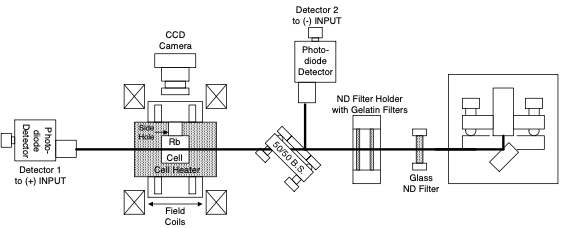
\includegraphics[width = .48\textwidth]{"content/pics/Aufbau.png"}
    \caption{Der Aufbau des Versuches \cite{v48}.}
    \label{fig:Aufbau}
\end{figure}
Zuerst wird die Probe mittels des Heizgerätes auf etwa $\qty{50}{\degreeCelsius}$ erhitzt und ein Spannung von $\qty{950}{\volt}$ an den Kondensator angelegt. 
Nach ca. $\qty{900}{\second}$ ist die Probe ausreichend polarisiert und die Heizung kann abgeschaltet werden. Flüssiger Stickstoff wird in das Dewar-Gefäß gefüllt, welcher 
die Probe über den Kupfer-Kühlfinger auf eine Temperatur von ungefähr $\qty{-60}{\degreeCelsius}$ herunter kühlt. Ist die Zieltemperatur erreicht, kann das elektrische Feld 
abgeschalten und der Kondensator über die Erdung des Amperemeters für einige Minuten entladen werden. Anschließend wird das Picoamperemeter angeschlossen. Über das Heizgerät wird die Probe langsam wieder auf 
$\qty{50}{\degreeCelsius}$ mit einer möglichst konstanten Heizrate erhitzt. Dabei wird jede Minute die Temperatur und der Depolarisationsstrom notiert.
Dieses Vorgehen wird für zwei unterschiedliche Heizraten $b$ (z.B. $b = 1,4 / \qty{2}{\degreeCelsius\per\minute}$) durchgeführt.
